%!TEX TS-program = xelatex
%!TEX encoding = UTF-8 Unicode
% Awesome CV LaTeX Template for CV/Resume
%
% This template has been downloaded from:
% https://github.com/posquit0/Awesome-CV
%
% Author:
% Claud D. Park <posquit0.bj@gmail.com>
% http://www.posquit0.com
%
%
% Adapted to be an Rmarkdown template by Mitchell O'Hara-Wild
% 23 November 2018
%
% Template license:
% CC BY-SA 4.0 (https://creativecommons.org/licenses/by-sa/4.0/)
%
%-------------------------------------------------------------------------------
% CONFIGURATIONS
%-------------------------------------------------------------------------------
% A4 paper size by default, use 'letterpaper' for US letter
\documentclass[11pt,a4paper,]{awesome-cv}

% Configure page margins with geometry
\usepackage{geometry}
\geometry{left=1.4cm, top=.8cm, right=1.4cm, bottom=1.8cm, footskip=.5cm}


% Specify the location of the included fonts
\fontdir[fonts/]

% Color for highlights
% Awesome Colors: awesome-emerald, awesome-skyblue, awesome-red, awesome-pink, awesome-orange
%                 awesome-nephritis, awesome-concrete, awesome-darknight

\definecolor{awesome}{HTML}{008080}

% Colors for text
% Uncomment if you would like to specify your own color
% \definecolor{darktext}{HTML}{414141}
% \definecolor{text}{HTML}{333333}
% \definecolor{graytext}{HTML}{5D5D5D}
% \definecolor{lighttext}{HTML}{999999}

% Set false if you don't want to highlight section with awesome color
\setbool{acvSectionColorHighlight}{true}

% If you would like to change the social information separator from a pipe (|) to something else
\renewcommand{\acvHeaderSocialSep}{\quad\textbar\quad}

\def\endfirstpage{\newpage}

%-------------------------------------------------------------------------------
%	PERSONAL INFORMATION
%	Comment any of the lines below if they are not required
%-------------------------------------------------------------------------------
% Available options: circle|rectangle,edge/noedge,left/right

\photo{../profile.png}
\name{Athanasia Monika Mowinckel}{}

\position{Staff Scientist}

\email{\href{mailto:a.m.mowinckel@psykologi.uio.no}{\nolinkurl{a.m.mowinckel@psykologi.uio.no}}}
\homepage{drmowinckels.io/}
\github{Athanasiamo}
\linkedin{drmowinckels}
\twitter{DrMowinckels}

% \gitlab{gitlab-id}
% \stackoverflow{SO-id}{SO-name}
% \skype{skype-id}
% \reddit{reddit-id}


\usepackage{booktabs}

\providecommand{\tightlist}{%
	\setlength{\itemsep}{0pt}\setlength{\parskip}{0pt}}

%------------------------------------------------------------------------------



% Pandoc CSL macros
\newlength{\cslhangindent}
\setlength{\cslhangindent}{1.5em}
\newlength{\csllabelwidth}
\setlength{\csllabelwidth}{3em}
\newenvironment{CSLReferences}[3] % #1 hanging-ident, #2 entry spacing
 {% don't indent paragraphs
  \setlength{\parindent}{0pt}
  % turn on hanging indent if param 1 is 1
  \ifodd #1 \everypar{\setlength{\hangindent}{\cslhangindent}}\ignorespaces\fi
  % set entry spacing
  \ifnum #2 > 0
  \setlength{\parskip}{#2\baselineskip}
  \fi
 }%
 {}
\usepackage{calc}
\newcommand{\CSLBlock}[1]{#1\hfill\break}
\newcommand{\CSLLeftMargin}[1]{\parbox[t]{\csllabelwidth}{#1}}
\newcommand{\CSLRightInline}[1]{\parbox[t]{\linewidth - \csllabelwidth}{#1}}
\newcommand{\CSLIndent}[1]{\hspace{\cslhangindent}#1}

\begin{document}

% Print the header with above personal informations
% Give optional argument to change alignment(C: center, L: left, R: right)
\makecvheader

% Print the footer with 3 arguments(<left>, <center>, <right>)
% Leave any of these blank if they are not needed
% 2019-02-14 Chris Umphlett - add flexibility to the document name in footer, rather than have it be static Curriculum Vitae
\makecvfooter
  {December, 2021}
    {Athanasia Monika Mowinckel~~~·~~~mowinckel\_cv}
  {\thepage}


%-------------------------------------------------------------------------------
%	CV/RESUME CONTENT
%	Each section is imported separately, open each file in turn to modify content
%------------------------------------------------------------------------------



\hypertarget{education}{%
\section{Education}\label{education}}

\begin{cventries}
    \cventry{Thesis title: Neurocognitive Processes of Decision-making in Adults with ADHD}{Philosofiae doctorem - University of Oslo - Norway}{}{2012 - 2016}{}\vspace{-4.0mm}
    \cventry{Thesis title: Default Mode Resting-State Functional Connectivity of the Aging Brain}{Master in Cognitive Neuroscience - University of Oslo - Norway}{}{2009 - 2011}{}\vspace{-4.0mm}
    \cventry{Thesis title: Attention Deficits in Mild Cognitive Impairment and Dementia of the Alzheimer Type}{Bachelor in Psychology - University of Oslo - Norway}{}{2006 - 2009}{}\vspace{-4.0mm}
\end{cventries}

\hypertarget{research-positions}{%
\section{Research positions}\label{research-positions}}

\begin{cventries}
    \cventry{Staff scientist}{University of Oslo - Center for Lifespan Changes in Brain and Cognition}{Oslo}{2018 - present}{\begin{cvitems}
\item Creation and maintenance of LCBC data-base
\item Data sharing and management in Lifebrain EU-project (WP2)
\item Oversee data quality in ongoing data-collection
\end{cvitems}}
    \cventry{Researcher / Project Manager}{University of Oslo - Center for Lifespan Changes in Brain and Cognition}{Oslo}{2016 - 2017}{\begin{cvitems}
\item Coordinating data collection, data-management, and research collaborations
\item Running analyses and data preparations
\end{cvitems}}
    \cventry{Research assistant and lab-technician}{University of Oslo - Dept. of Psychology}{Oslo}{2011 - 2012}{\begin{cvitems}
\item Work with functional MRI-analysis, supervising students, and transitioning lab from windows to a Linux
\item Scripting of experiments, testing of participants and work on application for grants and ethical approval
\end{cvitems}}
\end{cventries}

\hypertarget{memberships-services}{%
\section{Memberships \& Services}\label{memberships-services}}

\footnotesize

I am passionate about increasing the representation and retention of
women in science, and in improving the formal training and competencies
taught at the University. These interests are evident from task force
and board memberships, and in activities I engage in outside of work,
like R-Ladies.

\begin{cventries}
    \cventry{Global team member}{R-Ladies global team}{Oslo}{2019 - present}{\begin{cvitems}
\item Assisting in daily coordination and webpage maintenance of R-Ladies globally
\item Initiative running events for coding, networking and support of minority genders in the R-community
\end{cvitems}}
    \cventry{Co-founder and chair}{R-Ladies Oslo}{Oslo}{2018 - present}{\begin{cvitems}
\item Assisting in daily coordination and webpage maintenance of R-Ladies globally
\item Initiative running events for coding, networking and support of minority genders in the R-community
\end{cvitems}}
\end{cventries}\begin{cventries}
    \cventry{Member}{University of Oslo}{Oslo}{2019 - NA}{\begin{cvitems}
\item Dept. of Psychology internal ethics committee
\end{cvitems}}
    \cventry{Member }{University of Oslo}{Oslo}{2017 - 2018}{\begin{cvitems}
\item Task force proposing changes to the PhD-program
\end{cvitems}}
    \cventry{Member }{University of Oslo}{Oslo}{2016 - 2017}{\begin{cvitems}
\item Central task force regarding research ethics, GDPR, and Hospital/University collaboration
\end{cvitems}}
    \cventry{Faculty Board Member, elected}{University of Oslo}{Oslo}{2015 - 2015}{\begin{cvitems}
\item Faculty of Social Sciences
\end{cvitems}}
    \cventry{Department Board Member, elected}{University of Oslo}{Oslo}{2014 - 2015}{\begin{cvitems}
\item Dept. of Psychology
\end{cvitems}}
    \cventry{Co-founder and chair}{University of Oslo}{Oslo}{2013 - 2015}{\begin{cvitems}
\item PsyDoc - Interest organisation for PhDs and PostDocs.
\end{cvitems}}
\end{cventries}

\hypertarget{teaching-dissemination}{%
\section{Teaching \& Dissemination}\label{teaching-dissemination}}

\footnotesize

In addition to teaching and workshops, I run a coding and neuroscience
blog, \href{https://drmowinckels.io}{drmowinckels.io \faicon{globe} },
that includes tutorials in R and neuroimaging. I am also a certified
\href{https://software-carpentry.org/}{Software Carpentry Instructor \faicon{globe}}.

\hypertarget{university}{%
\subsection{University}\label{university}}

\begin{cventries}
    \cventry{Seminar teacher}{University of Oslo}{Oslo, Norway}{2012 - 2015}{\begin{cvitems}
\item Introduction to research methods (PSY1010/PSYC1100)
\item Experimental Cognitive Psychology (PSYC2102)
\end{cvitems}}
    \cventry{Supervisor}{University of Oslo}{Oslo, Norway}{2012 - 2015}{\begin{cvitems}
\item Bachelor thesis
\end{cvitems}}
    \cventry{Seminar teacher}{University of Oslo}{Oslo, Norway}{2009 - 2011}{\begin{cvitems}
\item Introduction to research methods (PSY1010/PSYC1100)
\item Introduction to social psychology (PSY1100)
\end{cvitems}}
\end{cventries}

\hypertarget{workshops}{%
\subsection{Workshops}\label{workshops}}

\begin{cventries}
    \cventry{Instructor}{Monthly internal R-workshops for LCBC}{Center for Lifespan Changes in Brain and Cognition}{Monthly 2018 - present}{\begin{cvitems}
\item 2 hour workshops in using R for analysis, visualization, dissemination etc.
\end{cvitems}}
    \cventry{Instructor}{Workshop: Straightforward introduction to mixed models \href{https://www.meetup.com/rladies-london/events/259655336/}{\faicon{globe}}}{Oslo UseR!}{June 5, 2019}{\begin{cvitems}
\item A short workshop in the use of Mixed-models for repeated measurement data
\end{cvitems}}
    \cventry{Instructor}{Linear Mixed models on repeated measurement data
\href{https://www.meetup.com/Oslo-useR-Group/events/260303778/}{\faicon{globe}}}{R-Ladies London}{March 28, 2019}{\begin{cvitems}
\item A short workshop in the use of Mixed-models for repeated measurement data
\end{cvitems}}
    \cventry{Co-instructor}{TidyVerse R \href{https://www.ub.uio.no/english/courses-events/courses/other/Carpentry/software-carpentry/time-and-place/180925-26_TidyR}{\faicon{globe}}}{University of Oslo - Software Carpentry}{Sept.  25 - 26, 2018}{\begin{cvitems}
\item Two-day workshop on using R and the Tidyverse-packages for data handling and analysis
\end{cvitems}}
\end{cventries}

\hypertarget{research-software-development}{%
\section{Research software
development}\label{research-software-development}}

\footnotesize

A recent interest and professional endeavor is creating R-packages to
improve data workflows and visualization in R. Icons link to package
websites with documentation (\faicon{globe}), and github repositories
(\faicon{github}) where source code is openly available.

\begin{cvhonors}
    \cvhonor{}{\textbf{ggseg \href{https://github.com/LCBC-UiO/ggseg}{\faicon{github}} \href{https://lcbc-uio.github.io/ggseg/}{\faicon{globe}}}: Lead developer \newline Visualization tool for brain atlas segmentations through R}{}{2018 - present}
    \cvhonor{}{\textbf{ggeg3d \href{https://github.com/LCBC-UiO/ggseg3d}{\faicon{github}} \href{https://lcbc-uio.github.io/ggseg3d/}{\faicon{globe}}}: Lead developer \newline 3 dimensional visualization tool for brain atlas segmentations through R}{}{2018 - present}
    \cvhonor{}{\textbf{ggegExtra \href{https://github.com/LCBC-UiO/ggsegExtra}{\faicon{github}} \href{https://lcbc-uio.github.io/ggsegExtra/}{\faicon{globe}}}: Lead developer \newline Repository of atlas data for the ggseg-packages}{}{2018 - present}
    \cvhonor{}{\textbf{nettskjemar \href{https://github.com/LCBC-UiO/nettskjemar}{\faicon{github}} \href{https://lcbc-uio.github.io/nettskjemar/}{\faicon{globe}}}: Lead developer \newline Package to retrieve data and meta-data from the nettskjema questionnaire tool developed by the University of Oslo}{}{2019 - present}
    \cvhonor{}{\textbf{metagam \href{https://github.com/Lifebrain/metagam}{\faicon{github}} \href{https://lifebrain.github.io/metagam/}{\faicon{globe}}}: Contributor \newline Meta-Analysis of Generalized Additive Models in Neuroimaging Studies}{}{2020}
\end{cvhonors}

\newpage

\hypertarget{publications-preprints}{%
\section{Publications \& Preprints}\label{publications-preprints}}

In descending chronological order.

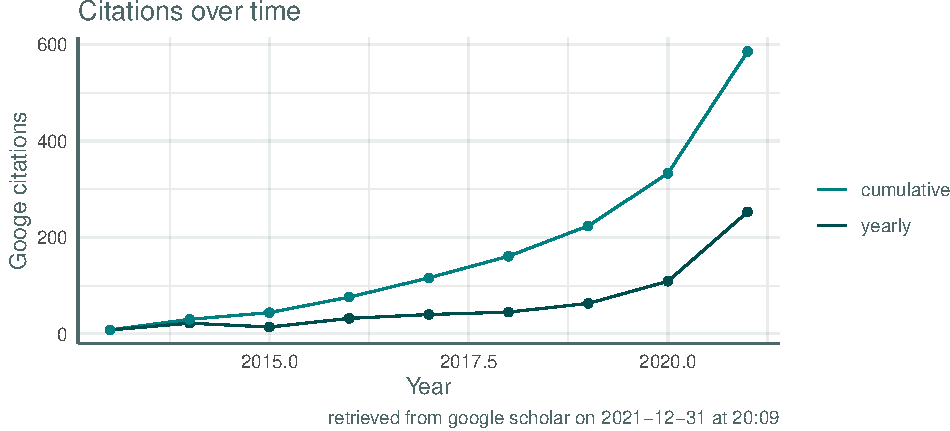
\includegraphics[width=1\linewidth]{am_mowinckel_cv_files/figure-latex/pubPlot-1}

\begin{cvhonors}
    \cvhonor{}{JM Roe, D Vidal-Piñeiro, Ø Sørensen, AM Brandmaier, S Düzel, et al. \newline \textit{Asymmetric thinning of the cerebral cortex across the adult lifespan is accelerated in Alzheimer’s disease} \newline \href{https://scholar.google.no/scholar?oi=bibs&hl=en&cluster=13796097502565679485}{Nature communications 12 1 111} \vspace{1mm} }{cites: 10}{2021}
    \cvhonor{}{KB Walhovd, AM Fjell, Y Wang, IK Amlien, AM \textbf{Mowinckel}, et al. \newline \textit{Education and Income Show Heterogeneous Relationships to Lifespan Brain and Cognitive Differences Across European and US Cohorts.} \newline \href{https://scholar.google.no/scholar?oi=bibs&hl=en&cluster=9119756821592181573}{Oxford University Press (OUP)  } \vspace{1mm} }{cites: 5}{2021}
    \cvhonor{}{AM Fjell, Ø Sørensen, IK Amlien, D Bartrés-Faz, AM Brandmaier, et al. \newline \textit{Poor Self-Reported Sleep is Related to Regional Cortical Thinning in Aging but not Memory Decline—Results From the Lifebrain Consortium} \newline \href{https://scholar.google.no/scholar?oi=bibs&hl=en&cluster=9441074857676075259}{Cerebral Cortex 31 4 19531969} \vspace{1mm} }{cites: 5}{2021}
    \cvhonor{}{Ø Sørensen, AM Brandmaier, D Macià, K Ebmeier, P Ghisletta, RA Kievit, et al. \newline \textit{Meta-analysis of generalized additive models in neuroimaging studies} \newline \href{https://scholar.google.no/scholar?oi=bibs&hl=en&cluster=13042839360510237530}{NeuroImage 224 117416} \vspace{1mm} }{cites: 5}{2021}
    \cvhonor{}{AM Fjell, H Grydeland, Y Wang, IK Amlien, D Bartres-Faz, AM Brandmaier, et al. \newline \textit{The genetic organization of longitudinal subcortical volumetric change is stable throughout the lifespan} \newline \href{https://scholar.google.no/scholar?oi=bibs&hl=en&cluster=2400743366874587110,7119551764769195712}{Elife 10 e66466} \vspace{1mm} }{cites: 2}{2021}
    \cvhonor{}{D Vidal-Piñeiro, MH Sneve, IK Amlien, H Grydeland, AM \textbf{Mowinckel}, et al. \newline \textit{The functional foundations of episodic memory remain stable throughout the lifespan} \newline \href{https://scholar.google.no/scholar?oi=bibs&hl=en&cluster=6727128473922236992}{Cerebral Cortex 31 4 20982110} \vspace{1mm} }{cites: 1}{2021}
    \cvhonor{}{D Vidal-Pineiro, Y Wang, SK Krogsrud, IK Amlien, WFC Baare, et al. \newline \textit{Brain age relates to early life factors but not to accelerated brain aging} \newline \href{https://scholar.google.no/scholar?oi=bibs&hl=en&cluster=14333089339680091601,1074965980205397950}{BioRxiv  } \vspace{1mm} }{Preprint \newline cites: 1}{2021}
    \cvhonor{}{SK Krogsrud, AM \textbf{Mowinckel}, D Sederevicius, D Vidal-Piñeiro, IK Amlien, et al. \newline \textit{Relationships between apparent cortical thickness and working memory across the lifespan-Effects of genetics and socioeconomic status} \newline Developmental cognitive neuroscience 51 100997 \vspace{1mm} }{cites: 0}{2021}
    \cvhonor{}{AM \textbf{Mowinckel}, D Vidal-Piñeiro \newline \textit{Visualization of Brain Statistics With R Packages ggseg and ggseg3d} \newline \href{https://scholar.google.no/scholar?oi=bibs&hl=en&cluster=7728234467298477321}{Advances in Methods and Practices in Psychological Science 3 4 466483} \vspace{1mm} }{cites: 43}{2020}
    \cvhonor{}{D Vidal-Pineiro, N Parker, J Shin, L French, H Grydeland, AP Jackowski, et al. \newline \textit{Cellular correlates of cortical thinning throughout the lifespan} \newline \href{https://scholar.google.no/scholar?oi=bibs&hl=en&cluster=5860637791443459396}{Scientific Reports 10 1 114} \vspace{1mm} }{cites: 31}{2020}
    \cvhonor{}{AM Fjell, Ø Sørensen, IK Amlien, D Bartrés-Faz, DM Bros, N Buchmann, et al. \newline \textit{Self-reported sleep relates to hippocampal atrophy across the adult lifespan: results from the Lifebrain consortium} \newline \href{https://scholar.google.no/scholar?oi=bibs&hl=en&cluster=13478746394103686546}{Sleep 43 5 zsz280} \vspace{1mm} }{cites: 29}{2020}
    \cvhonor{}{KB Walhovd, AM Fjell, Ø Sørensen, AM \textbf{Mowinckel}, CS Reinbold, et al. \newline \textit{Genetic risk for Alzheimer disease predicts hippocampal volume through the human lifespan} \newline \href{https://scholar.google.no/scholar?oi=bibs&hl=en&cluster=2204833211052181607}{Neurology Genetics 6 5} \vspace{1mm} }{cites: 15}{2020}
\end{cvhonors}

\begin{cvhonors}
    \cvhonor{}{VM Danielsen, D Vidal-Piñeiro, AM \textbf{Mowinckel}, D Sederevicius, AM Fjell, et al. \newline \textit{Lifespan trajectories of relative corpus callosum thickness: regional differences and cognitive relevance} \newline \href{https://scholar.google.no/scholar?oi=bibs&hl=en&cluster=8904205061858122143}{Cortex 130 127141} \vspace{1mm} }{cites: 10}{2020}
    \cvhonor{}{I Budin-Ljøsne, BB Friedman, S Suri, C Solé-Padullés, S Düzel, et al. \newline \textit{The global brain health survey: development of a multi-language survey of public views on brain health} \newline \href{https://scholar.google.no/scholar?oi=bibs&hl=en&cluster=17972139162672856883}{Frontiers in public health 8 387} \vspace{1mm} }{cites: 2}{2020}
    \cvhonor{}{KB Walhovd, ACS Bråthen, MS Panizzon, AM \textbf{Mowinckel}, Ø Sørensen, et al. \newline \textit{Within-session verbal learning slope is predictive of lifespan delayed recall, hippocampal volume, and memory training benefit, and is heritable} \newline \href{https://scholar.google.no/scholar?oi=bibs&hl=en&cluster=8471967629941904538}{Scientific reports 10 1 113} \vspace{1mm} }{cites: 1}{2020}
    \cvhonor{}{AM Fjell, Ø Sørensen, IK Amlien, D Bartrés-Faz, AM Brandmaier, et al. \newline \textit{Self-reported sleep problems are related to cortical thinning in aging but not memory decline and amyloid-β accumulation–results from the Lifebrain consortium} \newline \href{https://scholar.google.no/scholar?oi=bibs&hl=en&cluster=9997302508201602939}{bioRxiv  } \vspace{1mm} }{Preprint \newline cites: 1}{2020}
    \cvhonor{}{AM Fjell, CH Chen, D Sederevicius, MH Sneve, H Grydeland, et al. \newline \textit{Continuity and discontinuity in human cortical development and change from embryonic stages to old age} \newline \href{https://scholar.google.no/scholar?oi=bibs&hl=en&cluster=12292935935753013374}{Cerebral Cortex 29 9 38793890} \vspace{1mm} }{cites: 18}{2019}
    \cvhonor{}{D Vidal-Piñeiro, MH Sneve, LH Nyberg, AM \textbf{Mowinckel}, D Sederevicius, et al. \newline \textit{Maintained frontal activity underlies high memory function over 8 years in aging} \newline \href{https://scholar.google.no/scholar?oi=bibs&hl=en&cluster=17089103347718824083}{Cerebral Cortex 29 7 31113123} \vspace{1mm} }{cites: 17}{2019}
    \cvhonor{}{AM Fjell, MH Sneve, D Sederevicius, Ø Sørensen, SK Krogsrud, et al. \newline \textit{Volumetric and microstructural regional changes of the hippocampus underlying development of recall performance after extended retention intervals} \newline \href{https://scholar.google.no/scholar?oi=bibs&hl=en&cluster=6382077352973065340}{Developmental cognitive neuroscience 40 100723} \vspace{1mm} }{cites: 9}{2019}
    \cvhonor{}{KB Walhovd, AM Fjell, Ø Sørensen, AM \textbf{Mowinckel}, CS Reinbold, et al. \newline \textit{Genetic risk for Alzheimer’s disease predicts hippocampal volume through the lifespan} \newline \href{https://scholar.google.no/scholar?oi=bibs&hl=en&cluster=13849018663476393665}{bioRxiv 711689} \vspace{1mm} }{Preprint \newline cites: 5}{2019}
    \cvhonor{}{AM Fjell, MH Sneve, D Sederevicius, Ø Sørensen, SK Krogsrud, et al. \newline \textit{Volumetric and microstructural regional changes of the hippocampus underlying development of extended delay long-term memory} \newline \href{https://scholar.google.no/scholar?oi=bibs&hl=en&cluster=17521939232361433407}{bioRxiv 595827} \vspace{1mm} }{Preprint \newline cites: 1}{2019}
    \cvhonor{}{KB Walhovd, AM Fjell, R Westerhausen, L Nyberg, KP Ebmeier, et al. \newline \textit{Healthy minds 0–100 years: Optimising the use of European brain imaging cohorts (“Lifebrain”)} \newline \href{https://scholar.google.no/scholar?oi=bibs&hl=en&cluster=761121902853026504}{European Psychiatry 50 4756} \vspace{1mm} }{cites: 36}{2018}
    \cvhonor{}{D Vidal-Piñeiro, SH Markus, L Nyberg, AM \textbf{Mowinckel}, D Sederevicius, et al. \newline \textit{P2‐395: TESTING MAINTENANCE AND COMPENSATION NOTIONS IN NORMAL AGING: AGE‐RELATED CORRELATES OF ASSOCIATIVE ENCODING SUCCESS} \newline Alzheimer's and Dementia 14 7SPart16 P854P854 \vspace{1mm} }{cites: 0}{2018}
    \cvhonor{}{AM \textbf{Mowinckel}, D Alnæs, ML Pedersen, S Ziegler, M Fredriksen, et al. \newline \textit{Increased default-mode variability is related to reduced task-performance and is evident in adults with ADHD} \newline \href{https://scholar.google.no/scholar?oi=bibs&hl=en&cluster=15217082774564824421}{NeuroImage: Clinical 16 369382} \vspace{1mm} }{cites: 37}{2017}
    \cvhonor{}{S Ziegler, ML Pedersen, AM \textbf{Mowinckel}, G Biele \newline \textit{Modelling ADHD: A review of ADHD theories through their predictions for computational models of decision-making and reinforcement learning} \newline \href{https://scholar.google.no/scholar?oi=bibs&hl=en&cluster=11108308558386894134}{Neuroscience and Biobehavioral Reviews 71 633656} \vspace{1mm} }{cites: 73}{2016}
    \cvhonor{}{AM \textbf{Mowinckel}, ML Pedersen, E Eilertsen, G Biele \newline \textit{A meta-analysis of decision-making and attention in adults with ADHD} \newline \href{https://scholar.google.no/scholar?oi=bibs&hl=en&cluster=9967029451223534628}{Journal of attention disorders 19 5 355367} \vspace{1mm} }{cites: 97}{2015}
    \cvhonor{}{AM \textbf{Mowinckel}, T Espeseth, LT Westlye \newline \textit{Network-specific effects of age and in-scanner subject motion: a resting-state fMRI study of 238 healthy adults} \newline \href{https://scholar.google.no/scholar?oi=bibs&hl=en&cluster=13651232777638540310}{Neuroimage 63 3 13641373} \vspace{1mm} }{cites: 139}{2012}
\end{cvhonors}



\end{document}
